\section{Jets}
\label{sec:jets}

Due to the confining nature of QCD, color-charged quarks and gluons produced in the
initial $pp$ interactions do not exist as free states for observably meaningful
timescales and therefore do not leave unambiguous signatures in the detector.
Instead, their production is characterised by the radiation of additional
quarks and gluons roughly collinear with the initiating colored particles.
The radiation pattern of these colored objects is dictated by the color field
that binds them and eventually results in the production of color-neutral hadrons.
The collimated spray of hadrons as a result of this \textit{hadronisation} process
leads to the phenomenology of \textit{jets}, which are the macroscopically observable signature
of produced quarks and gluons.
The reconstruction of jets refers to any suitable, i.e. physically meaningful and stable,
method for grouping together, or \textit{clustering}, the end-products of the hadronisation
process in such a way that the properites of the initiating quarks or gluons, such
as their quantum numbers and/or kinematics, can be inferred from the resulting clustered object.
The standard method for reconstructing jets in ATLAS will be introduced in Section~\ref{sec:jet_reco}.
In Section~\ref{sec:jet_calib}, the steps taken to turn these reconstructed jets into
accurate representations of the initiating quarks and/or gluons, so that they can
be used meaningfully in physics analyses, will be discussed.

\begin{figure}[!htb]
    \begin{center}
        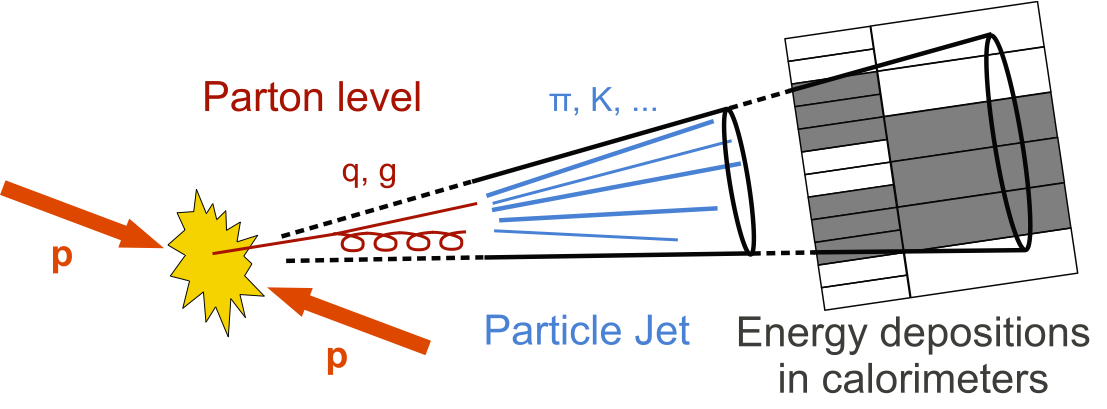
\includegraphics[width=0.7\textwidth]{figures/chapter3/jets/jet_formation_cartoon}
        \caption{
            Illustration of the jet formation process, beginning with the initiating quark and/or
            gluons (partons) which hadronise to form particle jets discernible by the tracking detectors
            in the ID and calorimeter jets defined by energy depositions in the calorimeter systems.
        }
        \label{fig:jet_formation}
    \end{center}
\end{figure}

\FloatBarrier
\subsection{Jet Reconstruction}
\label{sec:jet_reco}

\subsubsection{Topological Cell Clustering}
\label{sec:jet_topo_cluster}

The process of jet reconstruction begins first with the clustering of the lowest level calorimeter elements,
\textit{calorimeter cells}, corresponding to the readout channels in the LAr and tile calorimeters.
Figure~\ref{fig:calocell_granularity} gives an idea of the calorimeter cell granularity across the calorimeter
system.
The clustering algorithm used by ATLAS is a three-dimensional \textit{topological clustering} algorithm~\cite{Lampl:2008zz,Aad:2016upy}.
The highly granular calorimeter system used in ATLAS, with its finely segmented lateral readout and longitudinal sampling layers,
allows for the subsequent topological clusters (`topo-clusters') to capture in detail the energy-flow details of jets.
Topo-cluster formation begins by first identifying so-called \textit{seed cells} which have a rather high signal-to-noise ratio ($S/N$),
$S/N>4$.
Here, the signal is defined as the absolute value of the calorimter-cell energy measurement, $\lvert E \rvert$,
and the noise is defined as the sum in quadrature of the RMS of the electronics and expected pileup noise contributions.
Cells neighboring the seed cells satisfying $S/N>2$ are then collected into the topo-cluster.
A neighboring cell is defined in three-dimensions as either the calorimeter cells directly adjacent within the same calorimeter layer as
the seed cell, or, if in adjacent layers or in different calorimeter sub-systems, cells having at least partial overlap
in the $(\eta,\phi)$ plane with the seed.
The final set of cells, the perimeter cells, satisfying $S/N\ge0$ are then collected.
This last threshold essentially collects all those cells surrounding already-collected cells within each layer.
Figure~\ref{fig:calocell_clustering} illustrates the concept of topological cell clustering as described here.

\begin{figure}[!htb]
    \begin{center}
        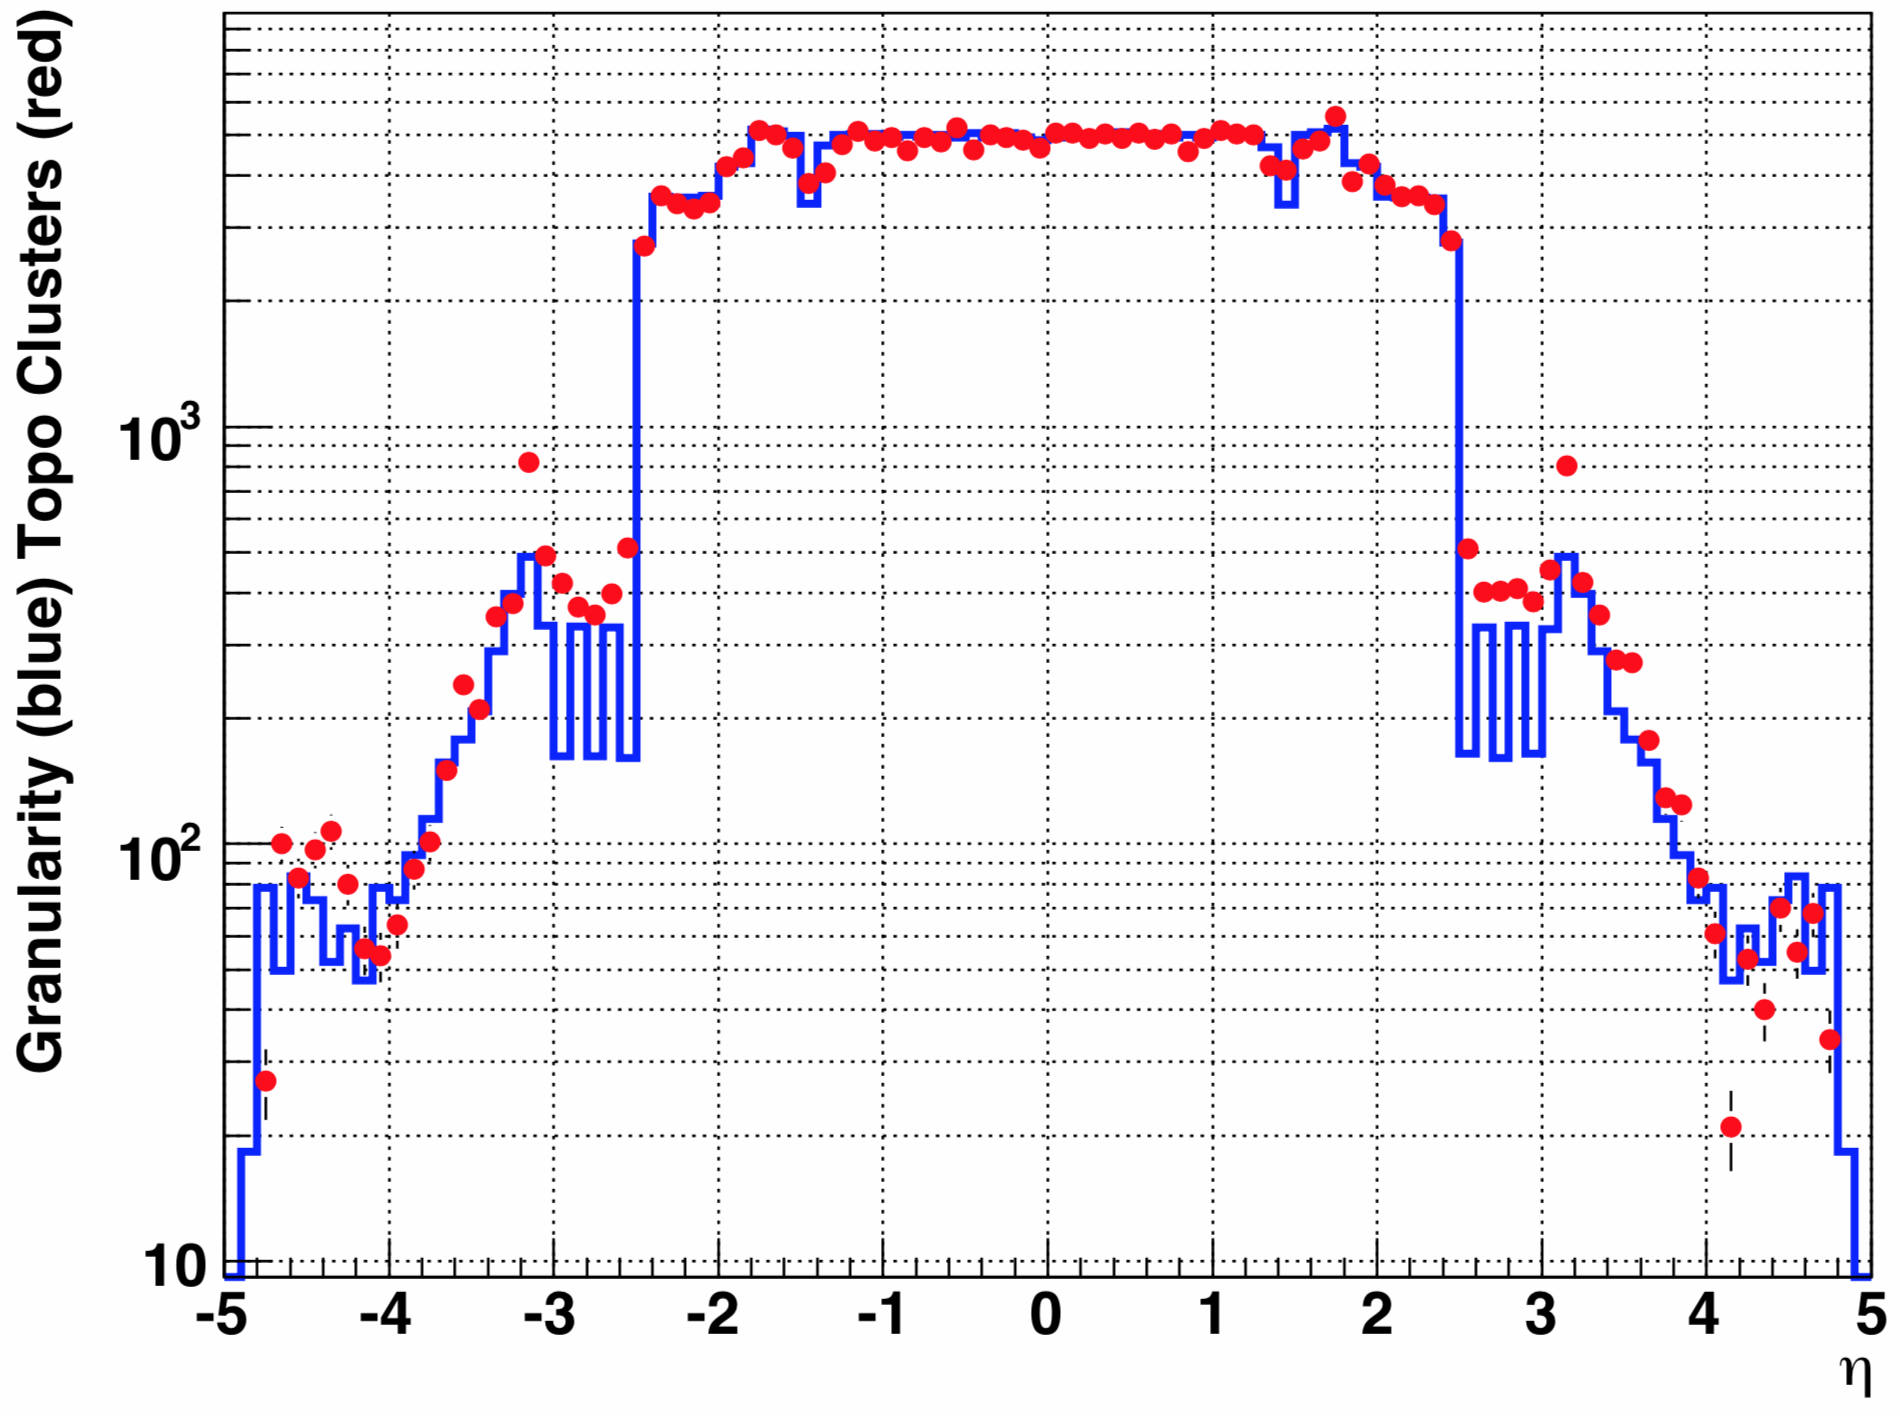
\includegraphics[width=0.5\textwidth]{figures/chapter3/jets/calocell_granularity}
        \caption{
            The blue histogram shows the average calorimeter cell granularity, i.e. number of calorimeter cells per
            $\Delta \eta = 0.1$, as a function of detector $\eta$. The red points show an approximation of the blue
            histogram based on calculations of the expected noise per calorimeter cell.
            From Ref.~\cite{Lampl:2008zz}.
        }
        \label{fig:calocell_granularity}
    \end{center}
\end{figure}

\begin{figure}[!htb]
    \begin{center}
    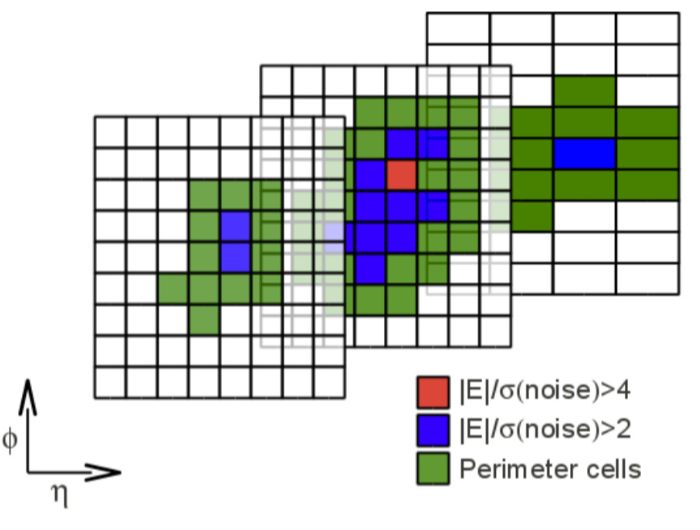
\includegraphics[width=0.6\textwidth]{figures/chapter3/jets/calocell_clustering_cartoon}
    \caption{
        Illustration of calorimeter-cell topological clustering across the three layers of the
        hadronic calorimeter. Indicated are the cells satisfying the signal-to-noise requirements for
        the seed (red), neighbor (blue), and perimeter (green) cells that make up the final three-dimensional topo-cluster.
    }
    \label{fig:calocell_clustering}
    \end{center}
\end{figure}
\FloatBarrier

\subsubsection{Jet Finding}
\label{sec:jet_finding}

Once the set of topo-clusters is formed, the process of jet finding begins.
As there is no single unique way to define a jet, there is a wide variety of jet finding algorithms whose
purpose is to associate jet constituents --- here, the calorimeter-cell topo-clusters --- to form
the final object representing the jet.
The default jet finding algorithm used by ATLAS is the
\textit{\antikt} jet clustering algorithm~\cite{Cacciari:2008gp}.
The \antikt~algorithm belongs to the more general class of sequential recombination algorithms
and is favored for its infrared and collinear (IRC) safe properties as well as the fact
that it tends to produce rather simple jets, geometrically, that are circular in the $\eta-\phi$ plane,
as seen in Figure~\ref{fig:antikt_circles}.
IRC safety in jet finding algorithms refers to the property that neither additional collinear splitting of jet constituents (e.g. the initiating or radiated partons)
nor soft emissions should change the clustered jet.
IRC-safe jets are therefore robust against these divergent regimes of QCD, sensitive to arbitrary
calculational choices made in perturbation theory, and makes them physically  meaningful observable objects
with which one can make predictions.

The \antikt algorithm takes as input constituents the topo-clusters described in Section~\ref{sec:jet_topo_cluster}
and computes the quantities,
\begin{align}
        d_{ij} = \min \left( \frac{1}{k^2_{T,i}} , \frac{1}{k^2_{T,j}} \right) \frac{ \Delta R_{ij}^2}{R^2},
        \label{eq:antikt_0}
\end{align}
\begin{align}
        d_{iB} = \frac{1}{k_{T,i}^2},
        \label{eq:antikt_1}
\end{align}
%with $\Delta R_{ij}^2 = (\eta_i - \eta_j)^2 + (\phi_i - \phi_j)^2$, {\color{red}{its rapidity, right?}} $R$ is a parameter whose value regulates the radial extent of
with $\Delta R_{ij}^2 = (y_i - y_j)^2 + (\phi_i - \phi_j)^2$, $R$ is a parameter whose value regulates the radial extent of
the jet, and $k_{T,i}$ is the transverse momentum of the $i^{th}$ constituent.
The $d_{ij}$ and $d_{iB}$ quantities are `distance' metrics used in the clustering of input topo-cluster constituents.
The former represents the `distance' between the $i^{th}$ and $j^{th}$ constituent while latter represents the
`distance' between the $i^{th}$ consituent and the beam-line, introduced to distinguish between constituents
originating from the primary hard-scatter vertex and those originating from soft proton interaction remnants.
The work to be discussed in the present thesis sets $R=0.4$, which is the standard used in ATLAS.

The \antikt algorithm proceeds by clustering those constituents whose inter-distance is smallest, thereby tending to cluster
higher-\pT constituents together, which can be seen by inspection of Equation~\ref{eq:antikt_0} and \ref{eq:antikt_1}.
If, of the set of input constituents, the smallest distance is a $d_{ij}$, the associated constituents indicated by $i$
and $j$ are recombined to form a single constituent in the list that replaces them both.
If the smallest distance is a $d_{iB}$, then the constituent indicated by index $i$ is removed from the set of constituents
and is considered as a complete jet.
This process repeats, starting with the now smaller (due to successful constituent recombination or removal) set of constituents,
until no constituents are left.
The result of this process is a set of recombined constituents that represent jets, as illustrated in Figure~\ref{fig:antikt_circles}.

\begin{figure}[!htb]
    \begin{center}
        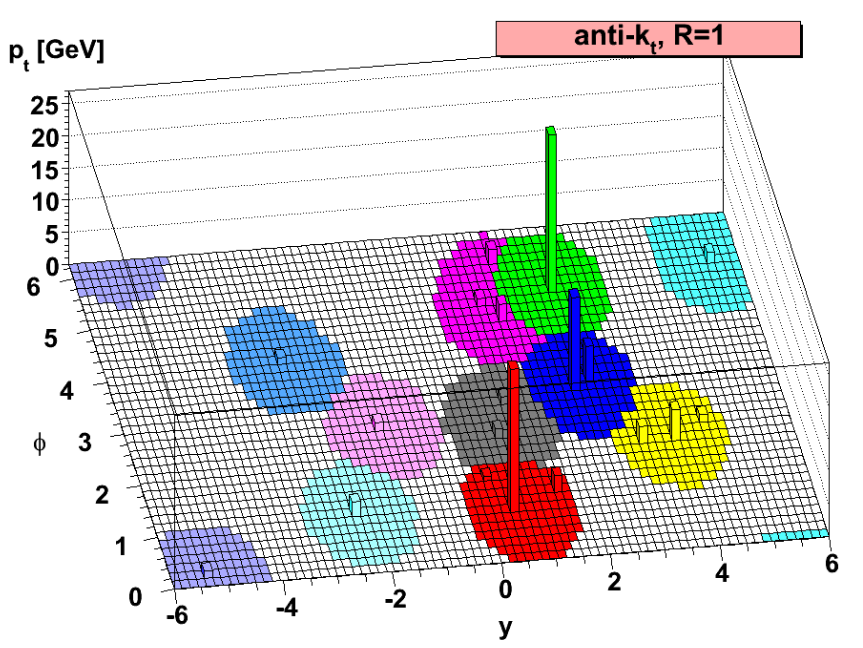
\includegraphics[width=0.5\textwidth]{figures/chapter3/jets/antikt_jet_circles}
        \caption{
            An illustration of jet constituents clustered by the \antikt~algorithm. Seen
            are the energetic constituents.
            The filled and colored circles represent areas populated by soft jet consituents, and represent the jet \textit{catchment area}~\cite{Cacciari:2008gn}
            whose size is dictated by the $R$ parameter in the \antikt algorithm (Equation~\ref{eq:antikt_0}).
            Figure taken from Ref.~\cite{Cacciari:2008gp}.
        }
        \label{fig:antikt_circles}
    \end{center}
\end{figure}

\FloatBarrier
%%%%%%%%%%%%%%%%%%%%%%%%%%%%%%%%%%%%%%%%%%%%%%%%%%%%%%%%%%%%%%%%%%%%%%%%%%%%%%%%%%%%%%%%%%%%%%%%%%
%%%%%%%%%%%%%%%%%%%%%%%%%%%%%%%%%%%%%%%%%%%%%%%%%%%%%%%%%%%%%%%%%%%%%%%%%%%%%%%%%%%%%%%%%%%%%%%%%%
%
% CALIBRATION
%
%%%%%%%%%%%%%%%%%%%%%%%%%%%%%%%%%%%%%%%%%%%%%%%%%%%%%%%%%%%%%%%%%%%%%%%%%%%%%%%%%%%%%%%%%%%%%%%%%%
%%%%%%%%%%%%%%%%%%%%%%%%%%%%%%%%%%%%%%%%%%%%%%%%%%%%%%%%%%%%%%%%%%%%%%%%%%%%%%%%%%%%%%%%%%%%%%%%%%


\subsection{Jet Calibration}
\label{sec:jet_calib}

\begin{figure}[!htb]
    \begin{center}
        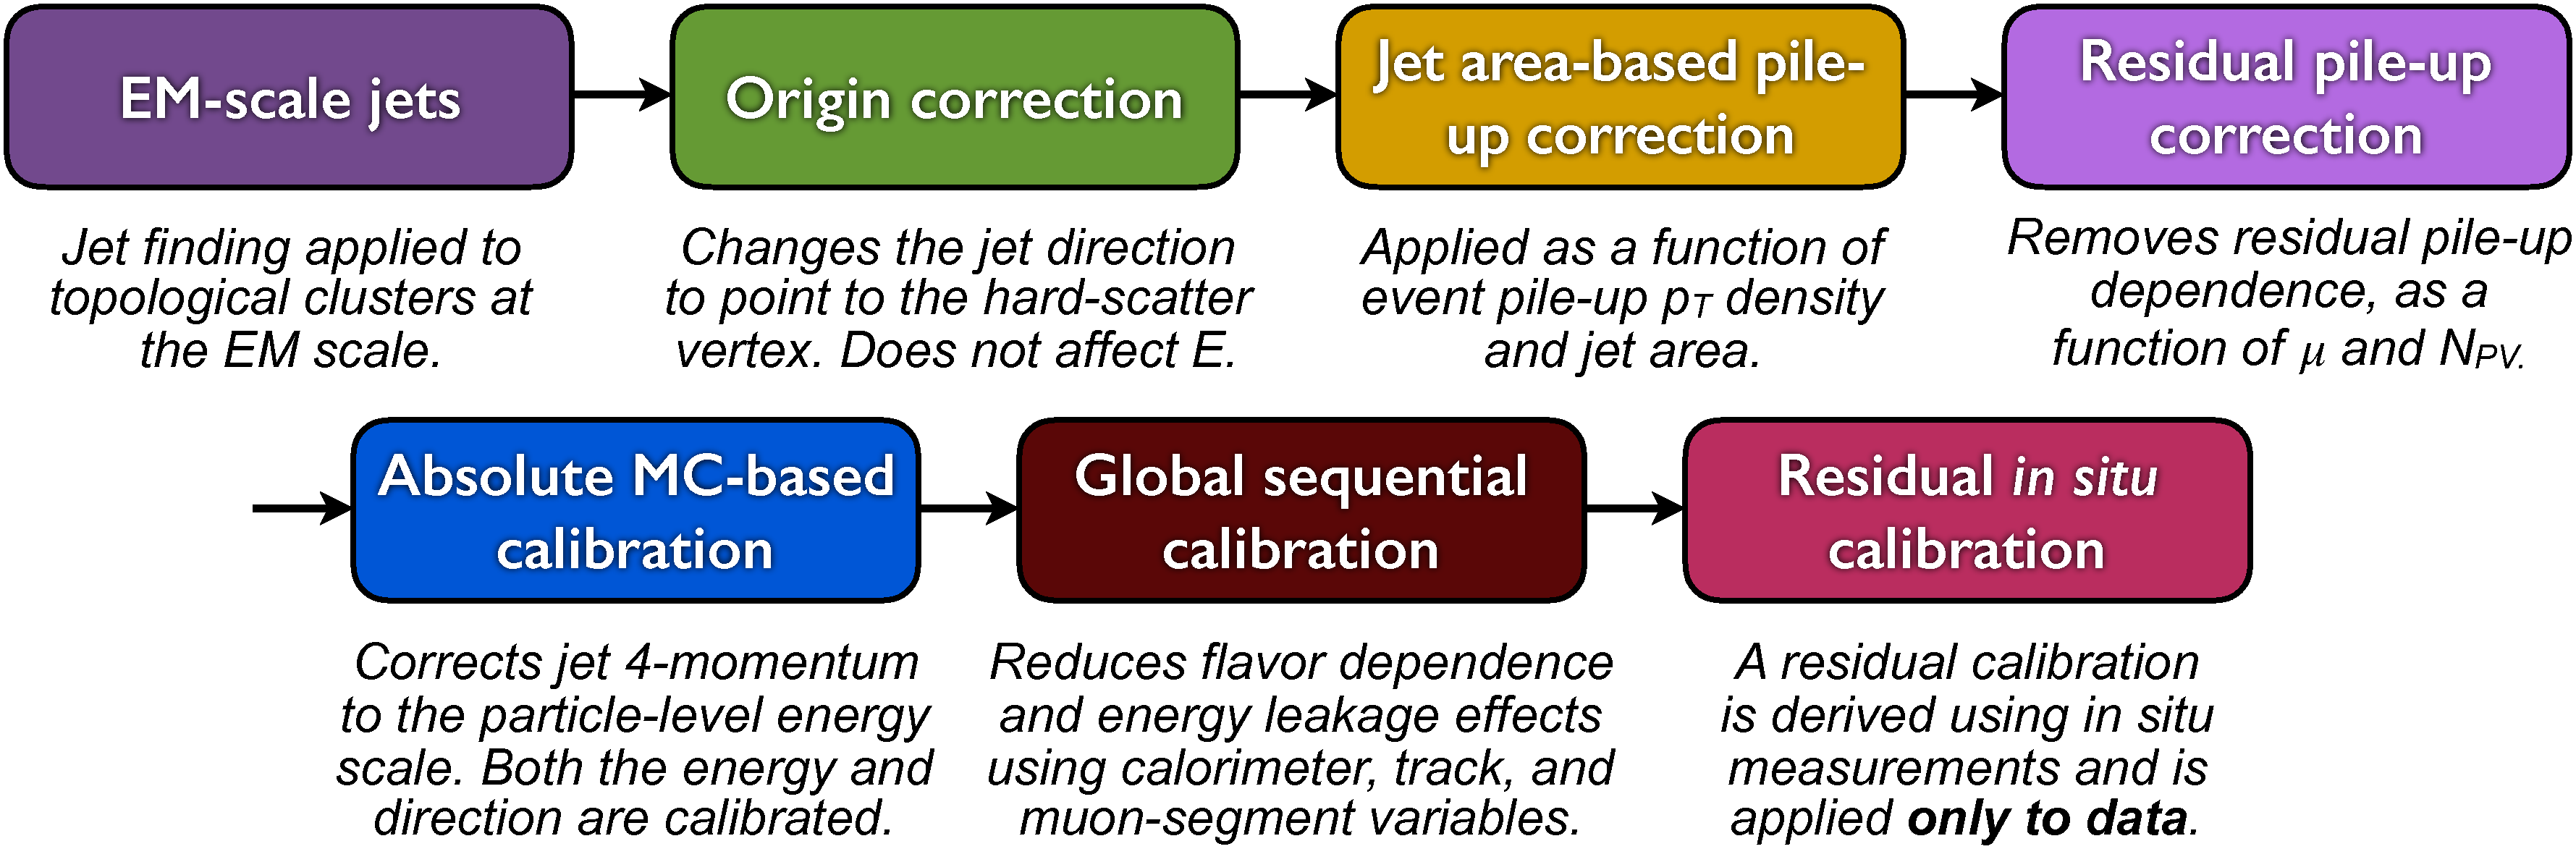
\includegraphics[width=0.8\textwidth]{figures/chapter3/jets/jes_calibration_sequence}
        \caption{
            Flowchart representing the sequence of steps taken in the jet calibration.
            From Ref.~\cite{Aaboud:2017jcu}.
        }
        \label{fig:jes_sequence}
    \end{center}
\end{figure}

The jets reconstructed following the steps described in Section~\ref{sec:jet_reco} are objects clustered
at the electromagnetic (EM) scale, which correctly measures the energy of electromagnetic showers but does not
accurately account for energy depositions characteristic of hadronic particle decays and interactions.
These jets are therefore referred to as `EM-scale' jets.
To correctly assign meaningful energy and momentum measurements to the reconstructed jets that correspond
to the energies and momenta of the initiating, underlying particle-level jets, several \textit{jet energy scale} (JES) calibration steps are taken~\cite{Aaboud:2017jcu}.
The steps are detailed in the flowchart in Figure~\ref{fig:jes_sequence} and will be briefly described in the following text.
The measurements made at each of these steps are subtle and account for many effects not present in the case
of the reconstruction of electrons and muons, for example, due to the fact that jets are rather complicated collective phenomena
whose measurements rely primarily on a single subsystem (the calorimeters).
Not only are electrons and muons generally simpler objects, seeded by comparatively unambiguous tracks within the ID,
their energy and momentum measurements are the result of a combination of well-defined measurements made by two independent
subsystems (ID measurements combined with EM calorimeter or the MS) that provide independent cross-checks on the validity
of the measurements made by each.
For the most part, this is not the case of the reconstruction of jets within ATLAS and as a result many of the choices made in the calibration
of EM-scale jets have non-negligible impact in the analyses that will be discussed in this thesis, whereas the analogous
choices for electrons and muons have minimal impact.
For this reason the jet calibration procedure outlined in Figure~\ref{fig:jes_sequence} will be outlined briefly in the text that follows.

\subsubsection{Jet Origin Correction}
\label{sec:jet_origin_correction}

The reconstructed EM-scale jets are built with the assumption that they originate from the geometric center
of the detector, as opposed to the primary hard-scatter vertex from which the initiating partons arise.
The so-called jet origin correction, therefore, refers to recalculating the jet four-momentum vector by adjusting it
in such a way that it points to the primary hard-scatter vertex.
This correction acts primarily to improve the $\eta$ resolution of jets.
This procedure is only one hundred percent accurate, of course, under the assumption that all of the jet constituents
going into the EM-scale jet reconstruction originated from the hard-scatter vertex, as opposed to some fraction having come from
a pileup vertex, for example.

\subsubsection{Pileup Corrections}
\label{sec:jet_pileup_correction}

Jets are extended object with relatively large \textit{catchment areas}~\cite{Cacciari:2008gn} that make them susceptible to
pileup effects.
Several corrections, therefore, to the jet energy are taken in order to account for contributions to the EM-scale jet reconstruction
arising from both in-time and out-of-time pileup interactions.

The first pileup correction is an area-based correction which subtracts the per-event pileup contribution to the
\pT~of each jet based on the jet's area, where the jet area is defined as in Ref.~\cite{Cacciari:2008gn}.
This pileup contribution is taken as the median \pT~density, $\rho$, of jets in the $\eta-\phi$ plane and
can be thought of as a baseline `noise' term distributed evenly throught the calorimeter that contributes to a jet's reconstructed energy.
%The quantity $\rho$ depends on the pileup activity in the event and is taken as a function of the number of reconstructed
%primary vertices (\npv) in a given event; for example, the pileup density is expected to be larger for an event
%with $\npv = 25$ as compared to one with $\npv = 5$.

After the area-based pileup correction is made, there still remains residual dependence of the reconstructed jet \pT~on the
number of reconstructed primary vertices and on the number of interactions, $\mu$.
These dependences are measured by performing linear fits of the jet \pT~as a function of each quantity, binned as a function of the detector $\eta$, $\eta_{\text{det}}$.

The final, pileup-corrected jet \pT~is given by Equation~\ref{eq:jet_pileup_corr}:
\begin{align}
    \pT^{\text{Corr}} = \pT^{\text{Reco}} - \underbrace{\rho \times A}_{\text{Area-based}} - \underbrace{\alpha \times (\npv - 1) - \beta \times \mu}_{\text{Residual}},
    \label{eq:jet_pileup_corr}
\end{align}
where $A$ is the jet area, and the $\alpha$ and $\beta$ terms are derived from the linear fits mentioned above and are $\alpha = \partial \pT / \partial \npv$
and $\beta = \partial \pT / \partial \mu$, respectively.
The former accounts for effects arising as a result of in-time pileup and the latter for those due to out-of-time pileup.
The effect of the pileup corrections is shown in Figure~\ref{fig:jet_pileup_corr}, where it can be seen that the area-based correction
is an overall offset, as expected, after which residual pileup dependencies of the jet \pT~as a function of $\lvert \eta_{\text{det}} \rvert$ are still observed.
This residual pileup dependence is greater in the forward regions of the detector where pileup and background activity is largest.

\begin{figure}[!htb]
    \begin{center}
        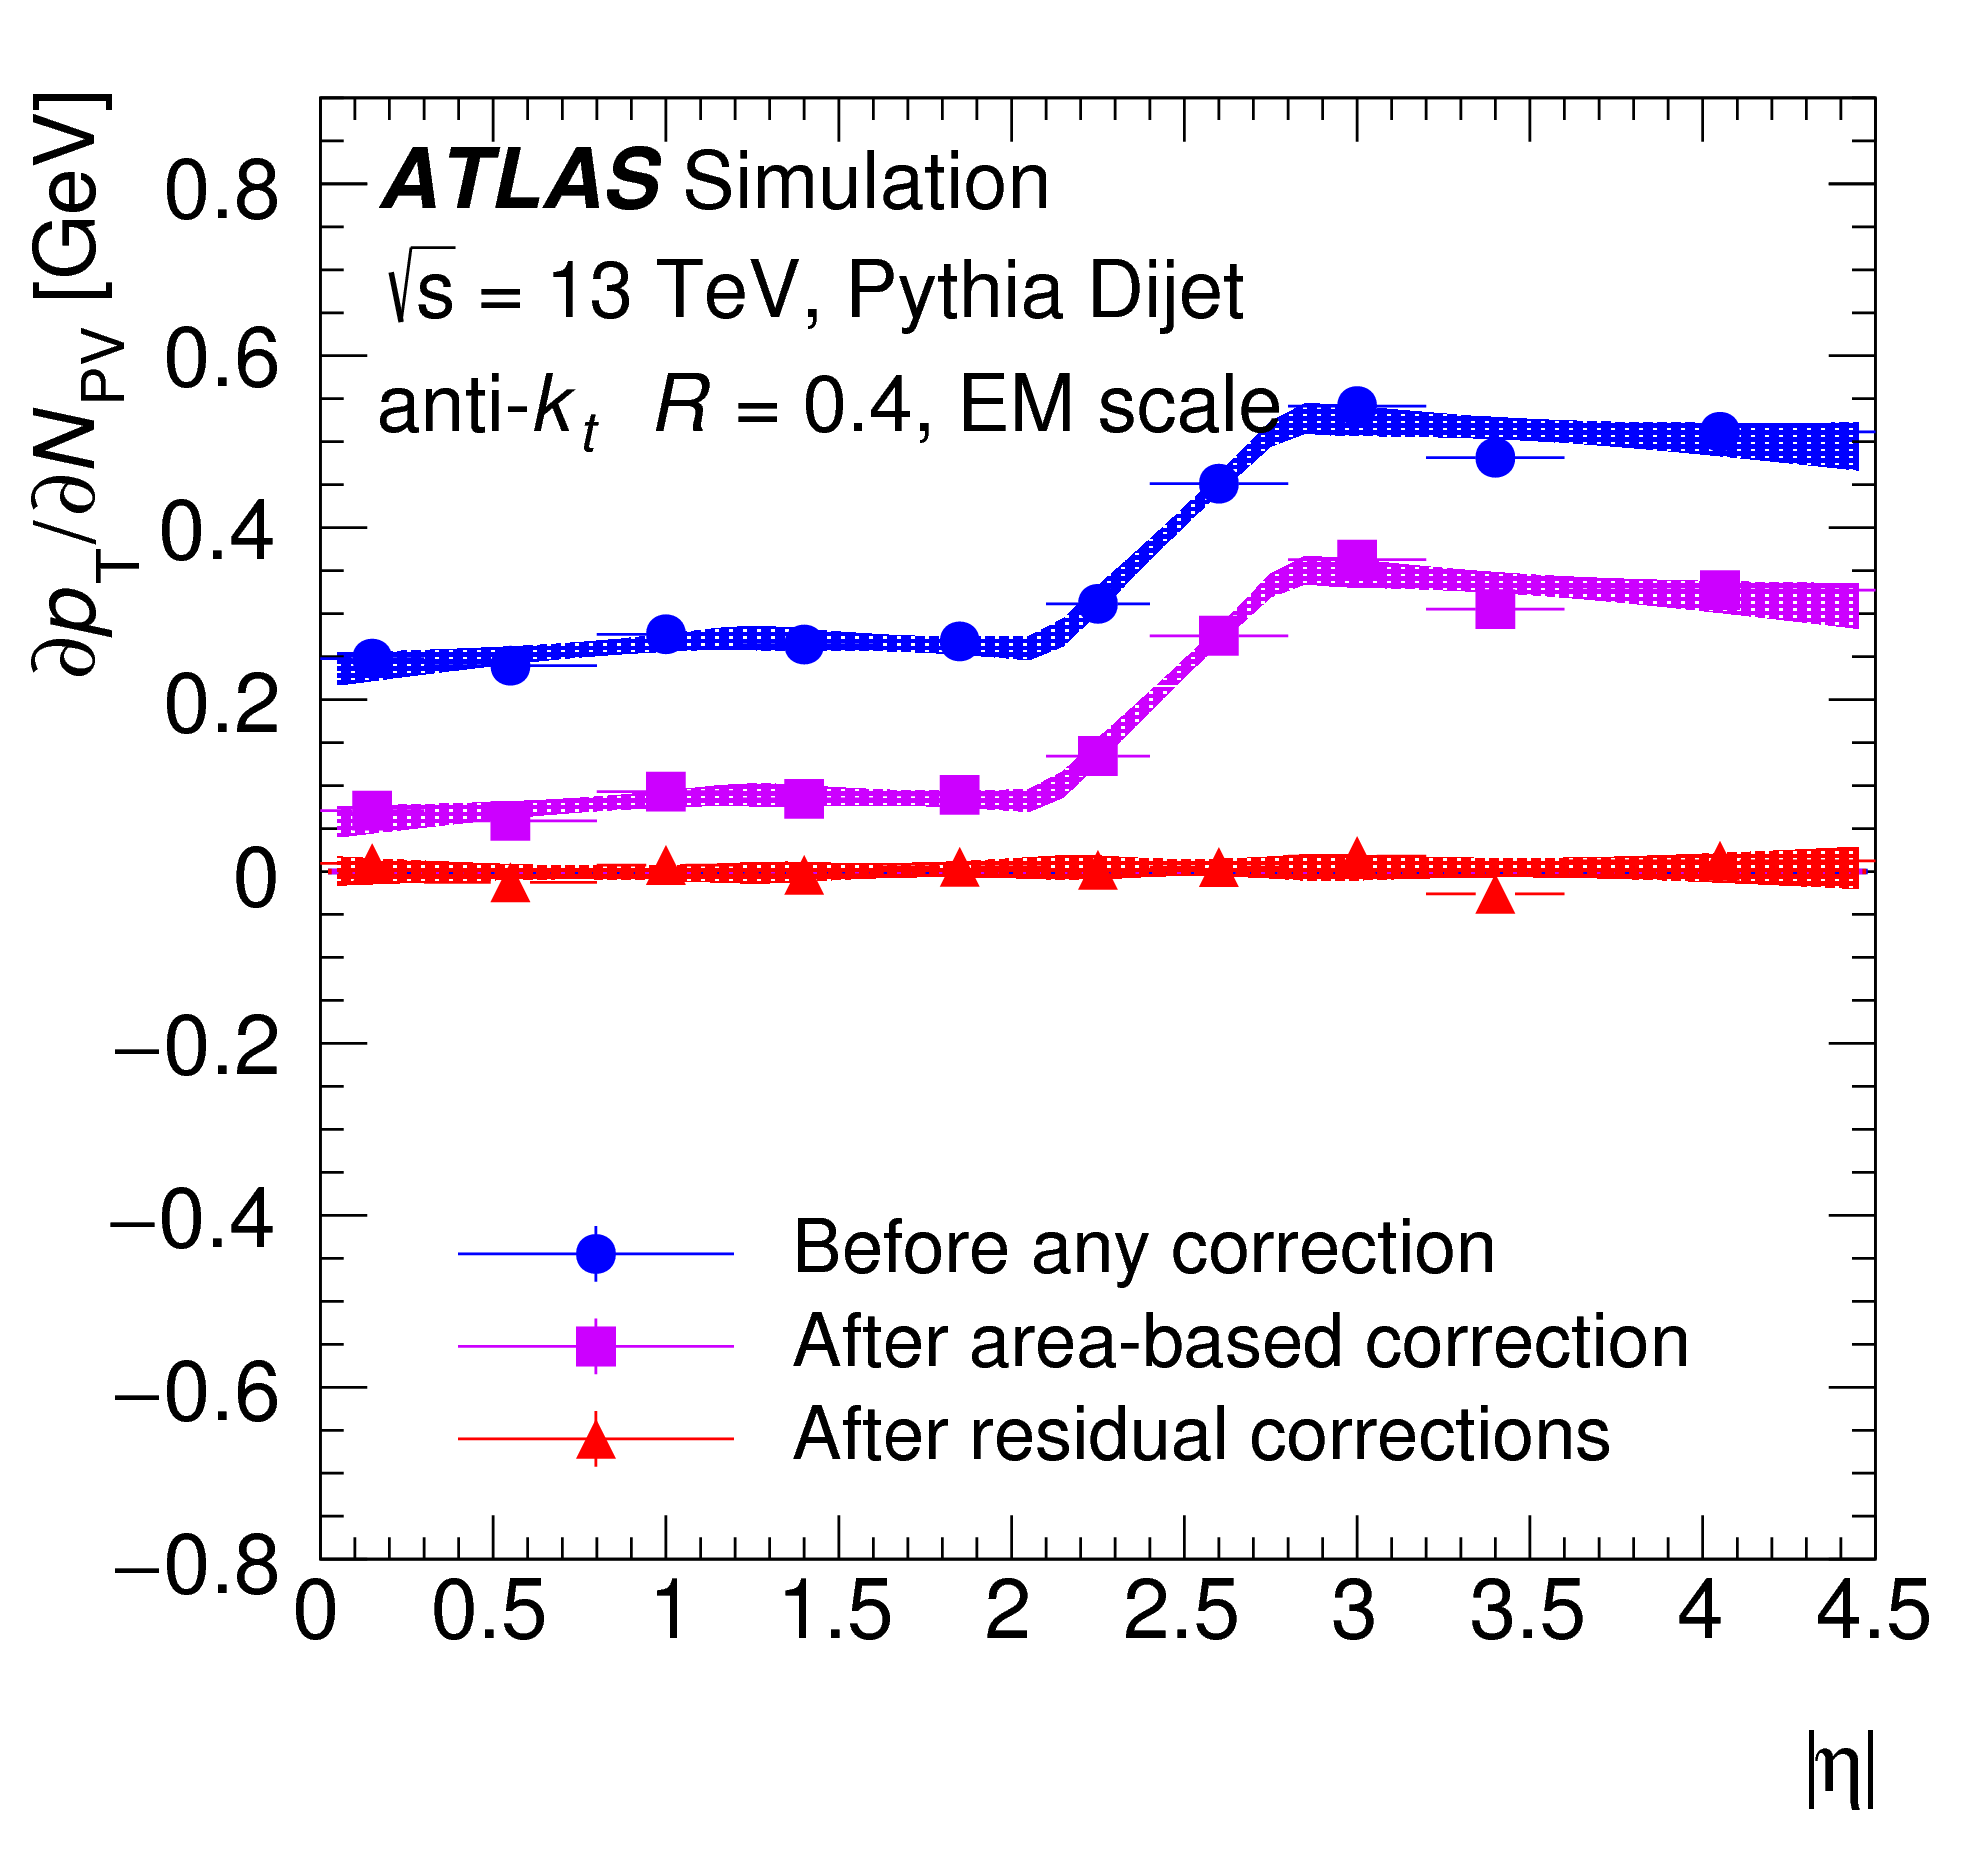
\includegraphics[width=0.4\textwidth]{figures/chapter3/jets/jet_pileup_corr_alpha}
        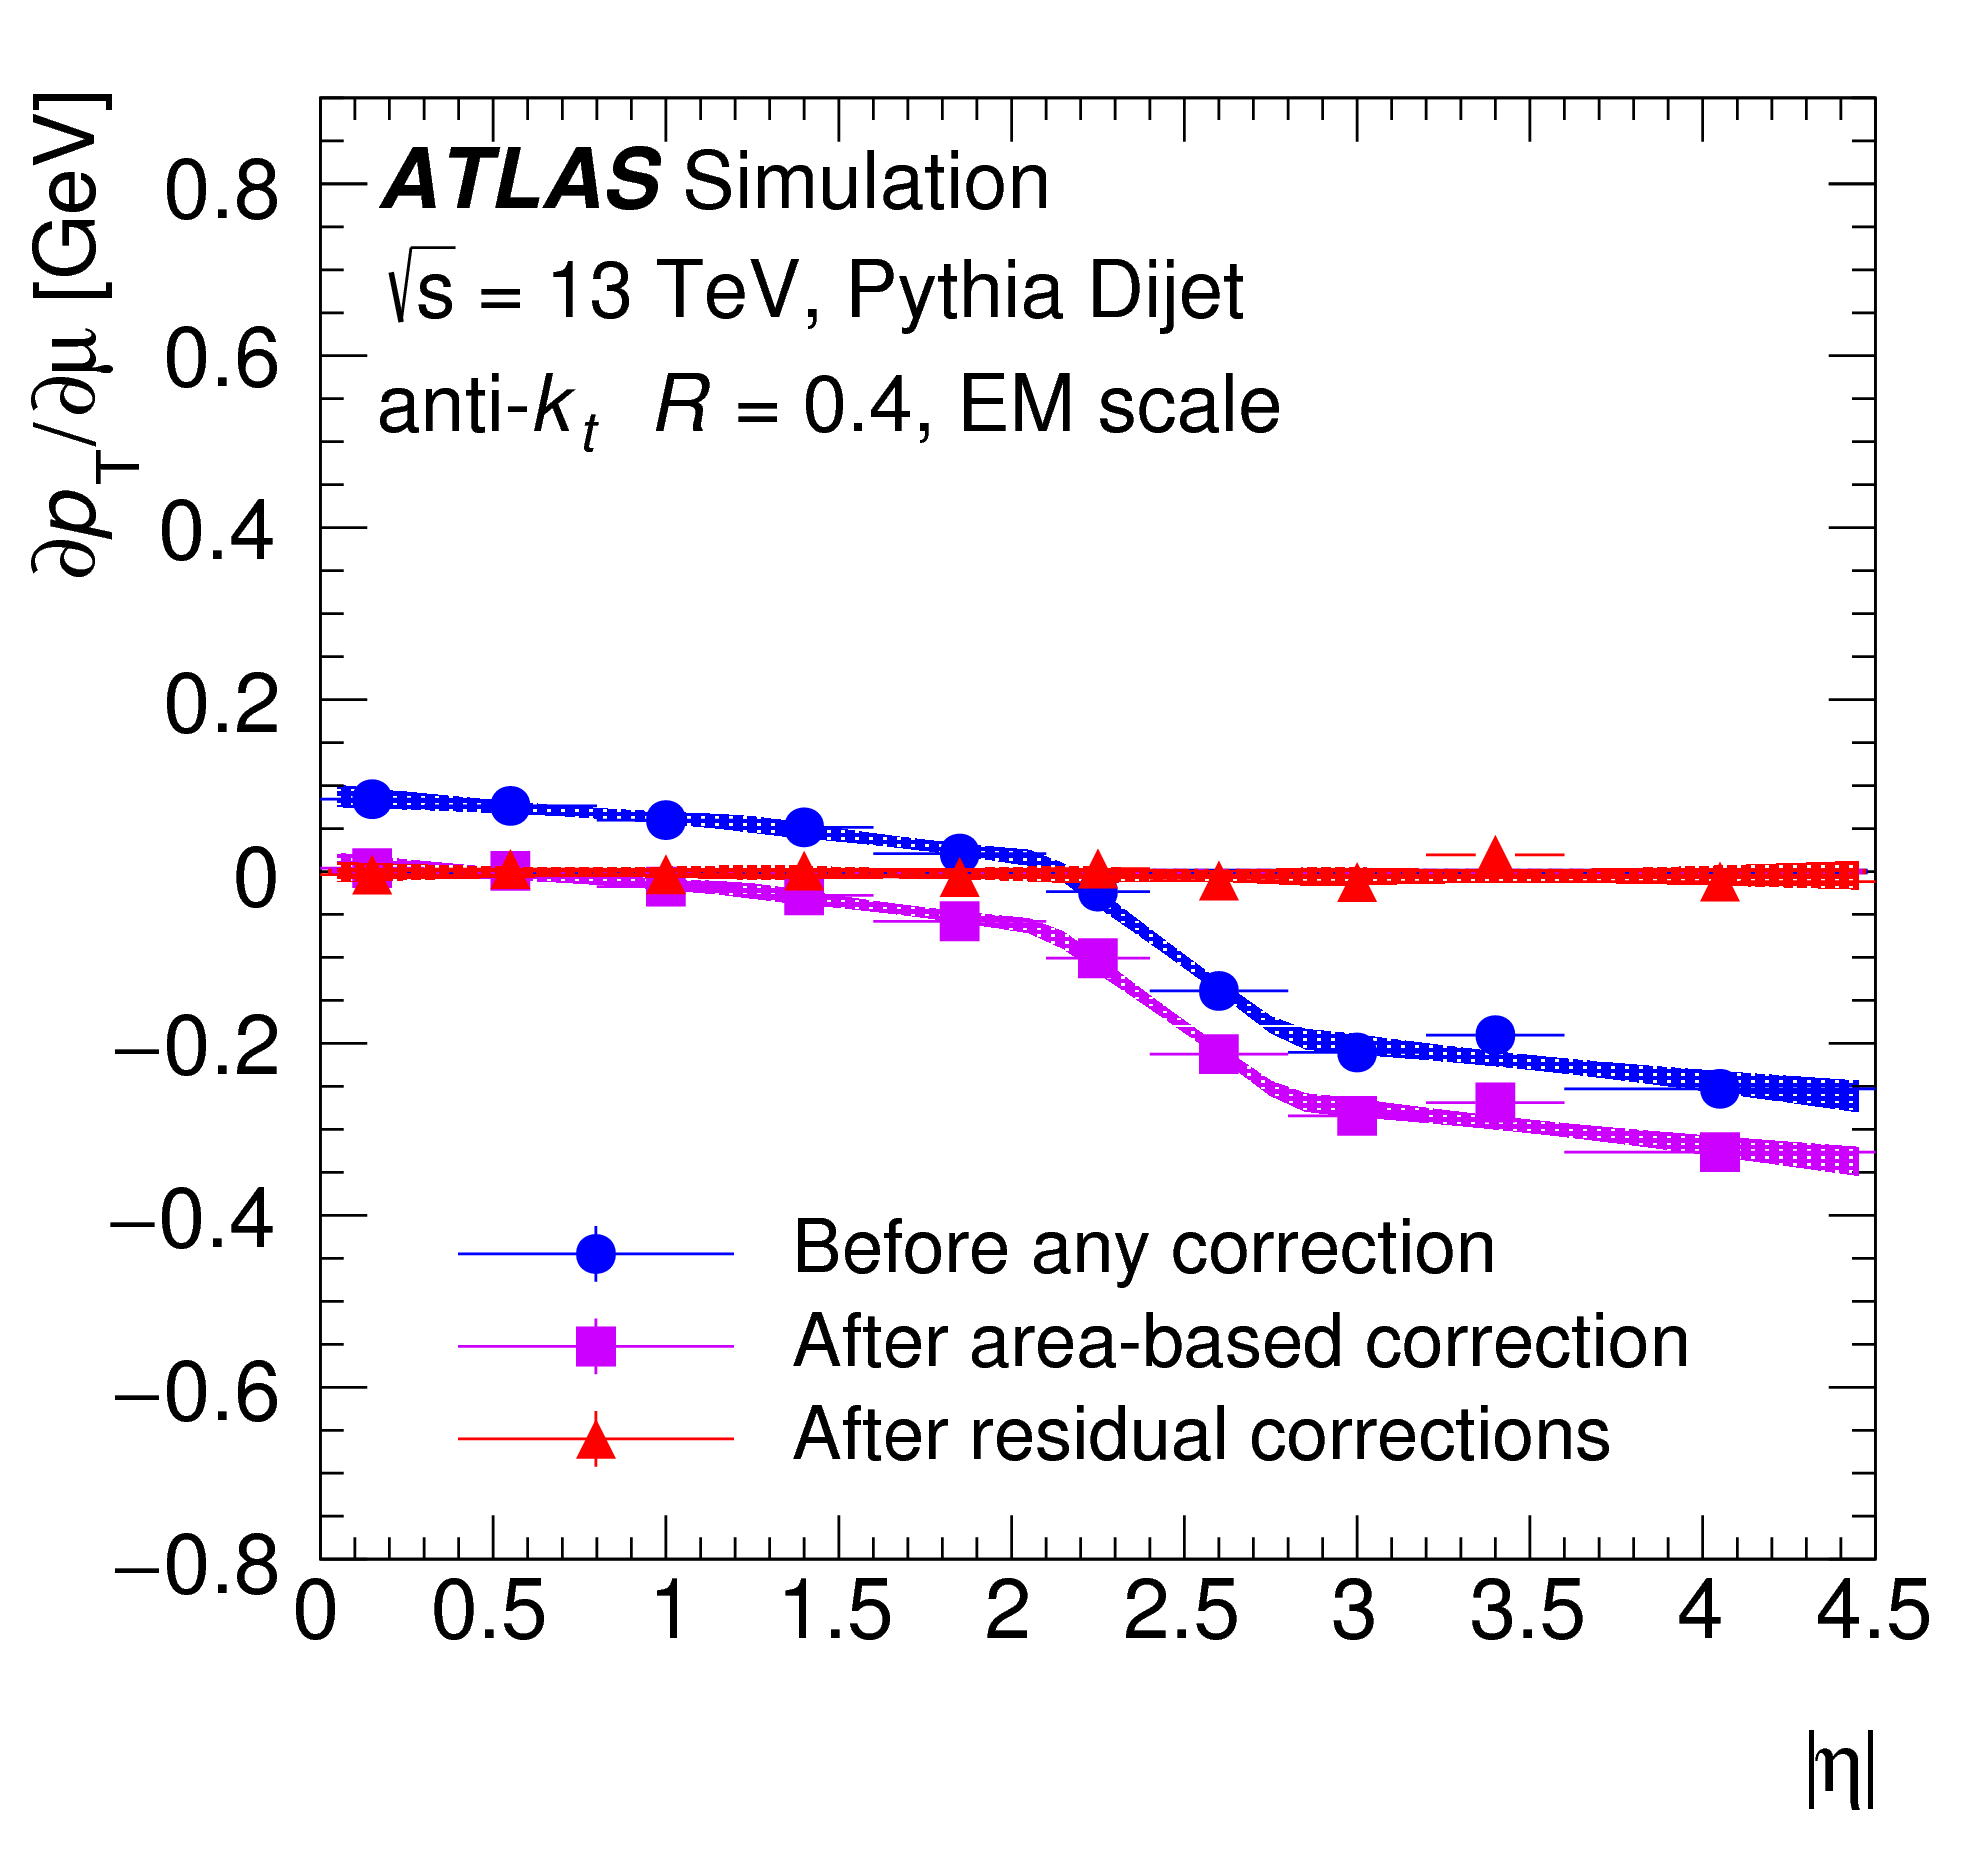
\includegraphics[width=0.4\textwidth]{figures/chapter3/jets/jet_pileup_corr_beta}
        \caption{
            Dependence of the \pT~of EM-scale reconstructed jets on \npv (in-time pileup) (\textbf{\textit{left}}) and on
            $\mu$ (out-of-time pileup) (\textbf{\textit{right}}).
            The blue curves show the dependence prior to any pileup corrections,
            the purple curves are after the area-based correction,
            and the red curves are the final dependence after the full pileup correction described in Equation~\ref{eq:jet_pileup_corr}
            is taken into account.
            Figures taken from Ref.~\cite{Aaboud:2017jcu}.
        }
        \label{fig:jet_pileup_corr}
    \end{center}
\end{figure}

\subsubsection{Absolute Jet Energy Scale and $\eta$ Correction}
\label{sec:jet_eta_corr}

This correction corrects the EM-scale reconstructed jet to the true energy scale based on particle-level
jets and is therefore purely MC-based.
Particle-level jets are jets clustered using the \antikt~algorithm using the generator-level
particles at the end of the hadronisation step as the input constituents, and therefore represent the reconstructed jet prior to
its interaction with the calorimeter (see Figure~\ref{fig:jet_formation}).
The correction accounts for mismodelling of the inactive material within the detector, radiation not accounted for
in the reconstructed calorimeter-based jet due to the clustering algorithm not accepting it (`out-of-cone radiation`),
non-compensation of the hadronic calorimeters, and for effects
%non-compensation of the hadronic calorimeters\footnote{ {\color{red}{Compensating...}}}, and for effects
related to detector geometry or transitions between calorimeter technologies.

The correction is derived by matching the EM-scale reconstructed jets, in simulation, to the particle-level
jets and deriving the average energy response, $E^{\text{Reco}} / E^{\text{Truth}}$, where $E^{\text{Truth}}$ is the
energy of the particle-level jet.
The inverse of this energy response is taken as a correction to the EM-scale reconstructed calorimeter jets in simulation.
An additional correction accounts for biases observed in the EM-scale reconstructed jet $\eta$, which is largest
in regions wherein a jet is likely to encompass two calorimeter regions or technologies which result in different
energy responses.
The $\eta$ correction is derived as the difference between the reconstructed and particle-level jet $\eta$ values and
applied to the EM-scale reconstructed calorimeter jets as in the case of the energy-response correction.
The average energy response, as a function of EM-scale jet \pT, and the $\eta$ correction is shown
in Figure~\ref{fig:abs_jes_response}.
After this correction stage, jets are referred to as being at the EM+JES scale.

\begin{figure}[!htb]
    \begin{center}
        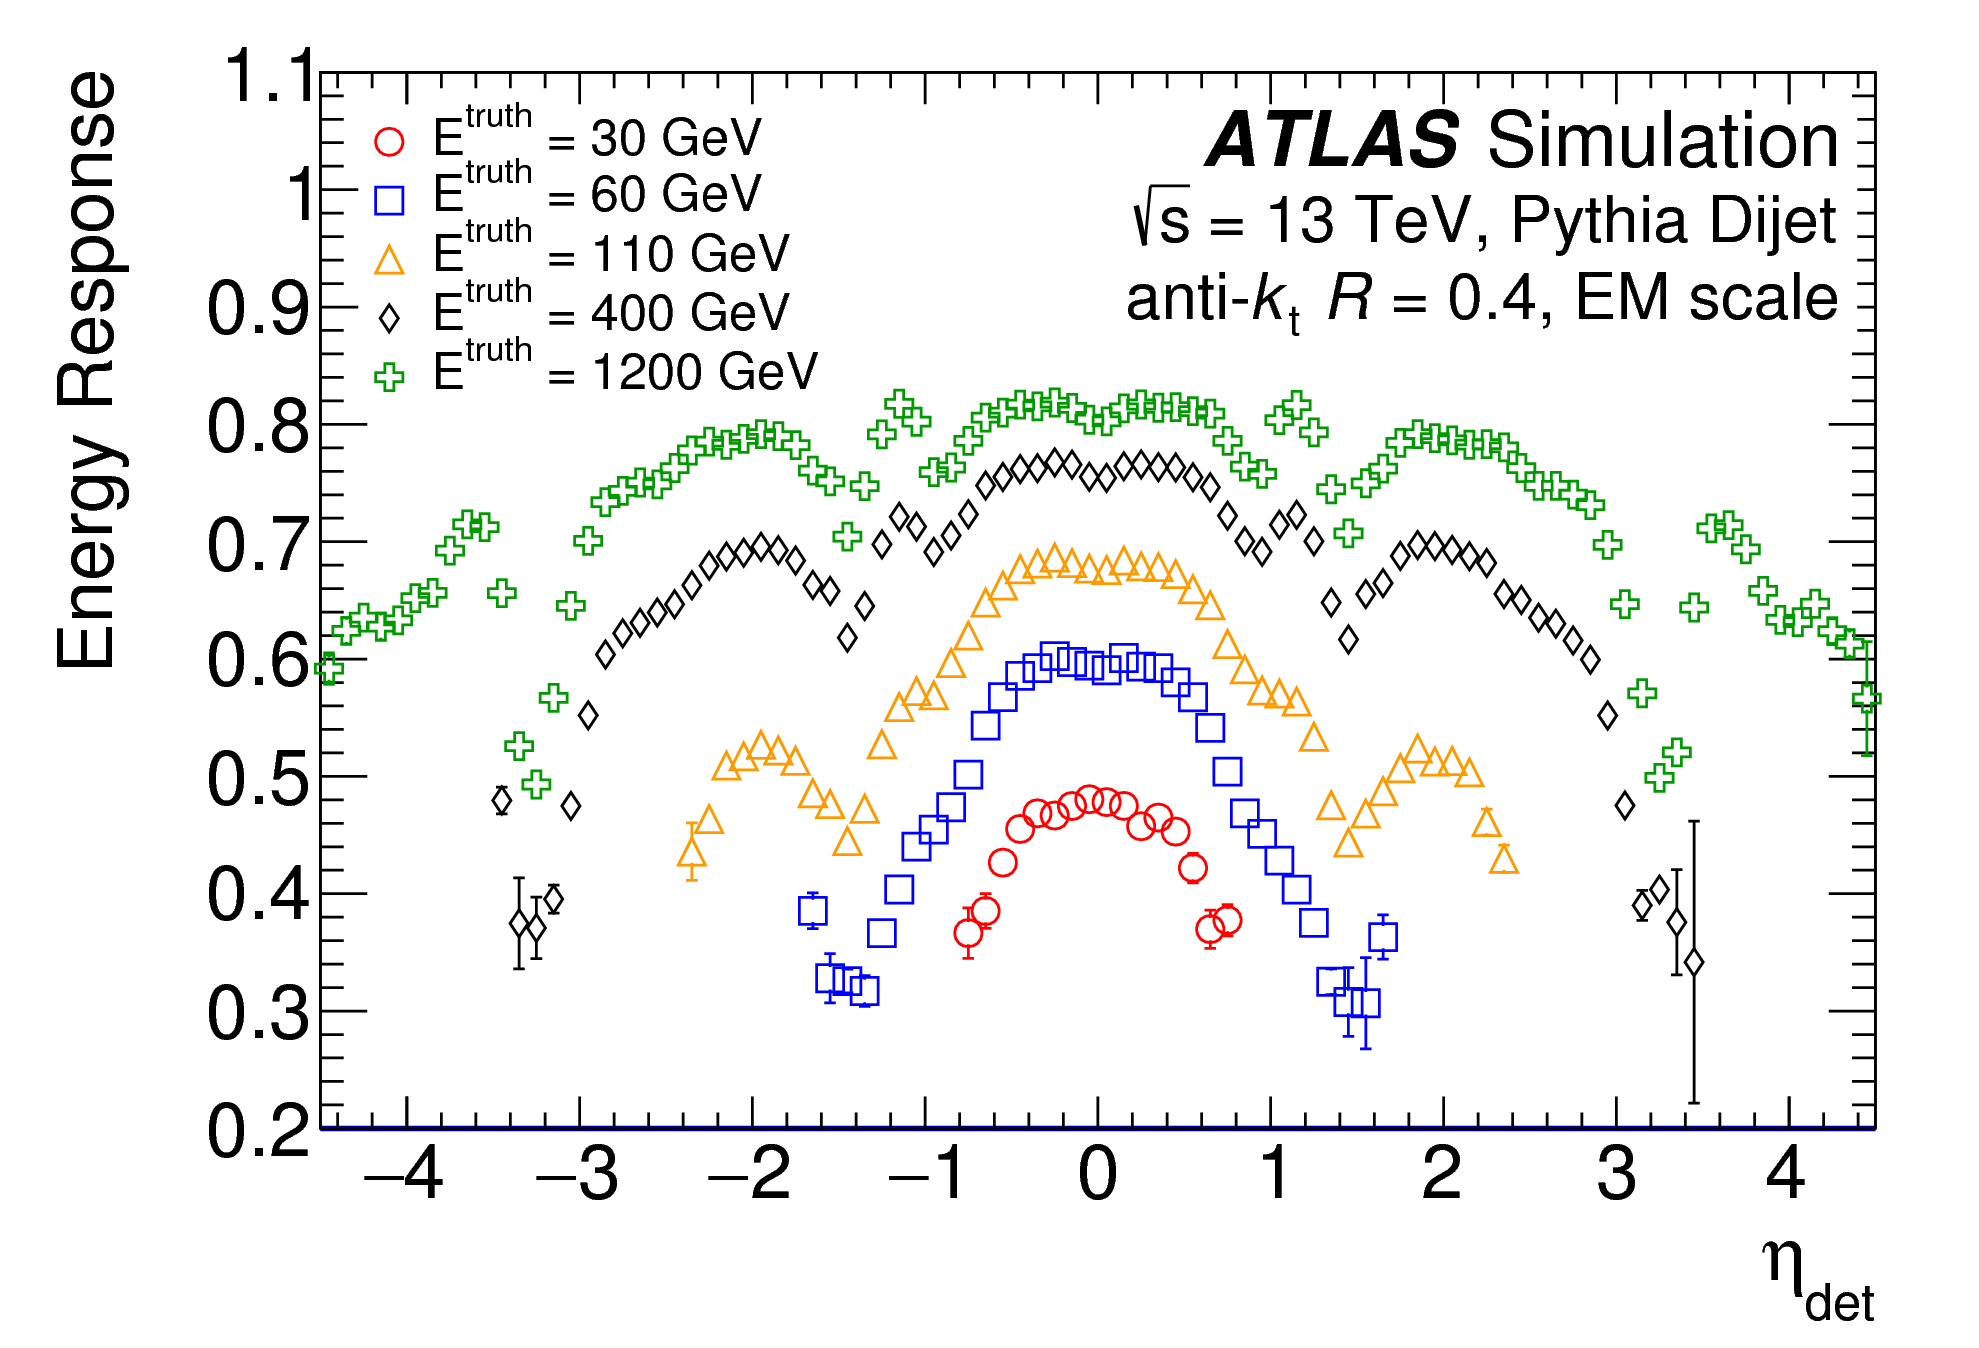
\includegraphics[width=0.48\textwidth]{figures/chapter3/jets/abs_jes_response}
        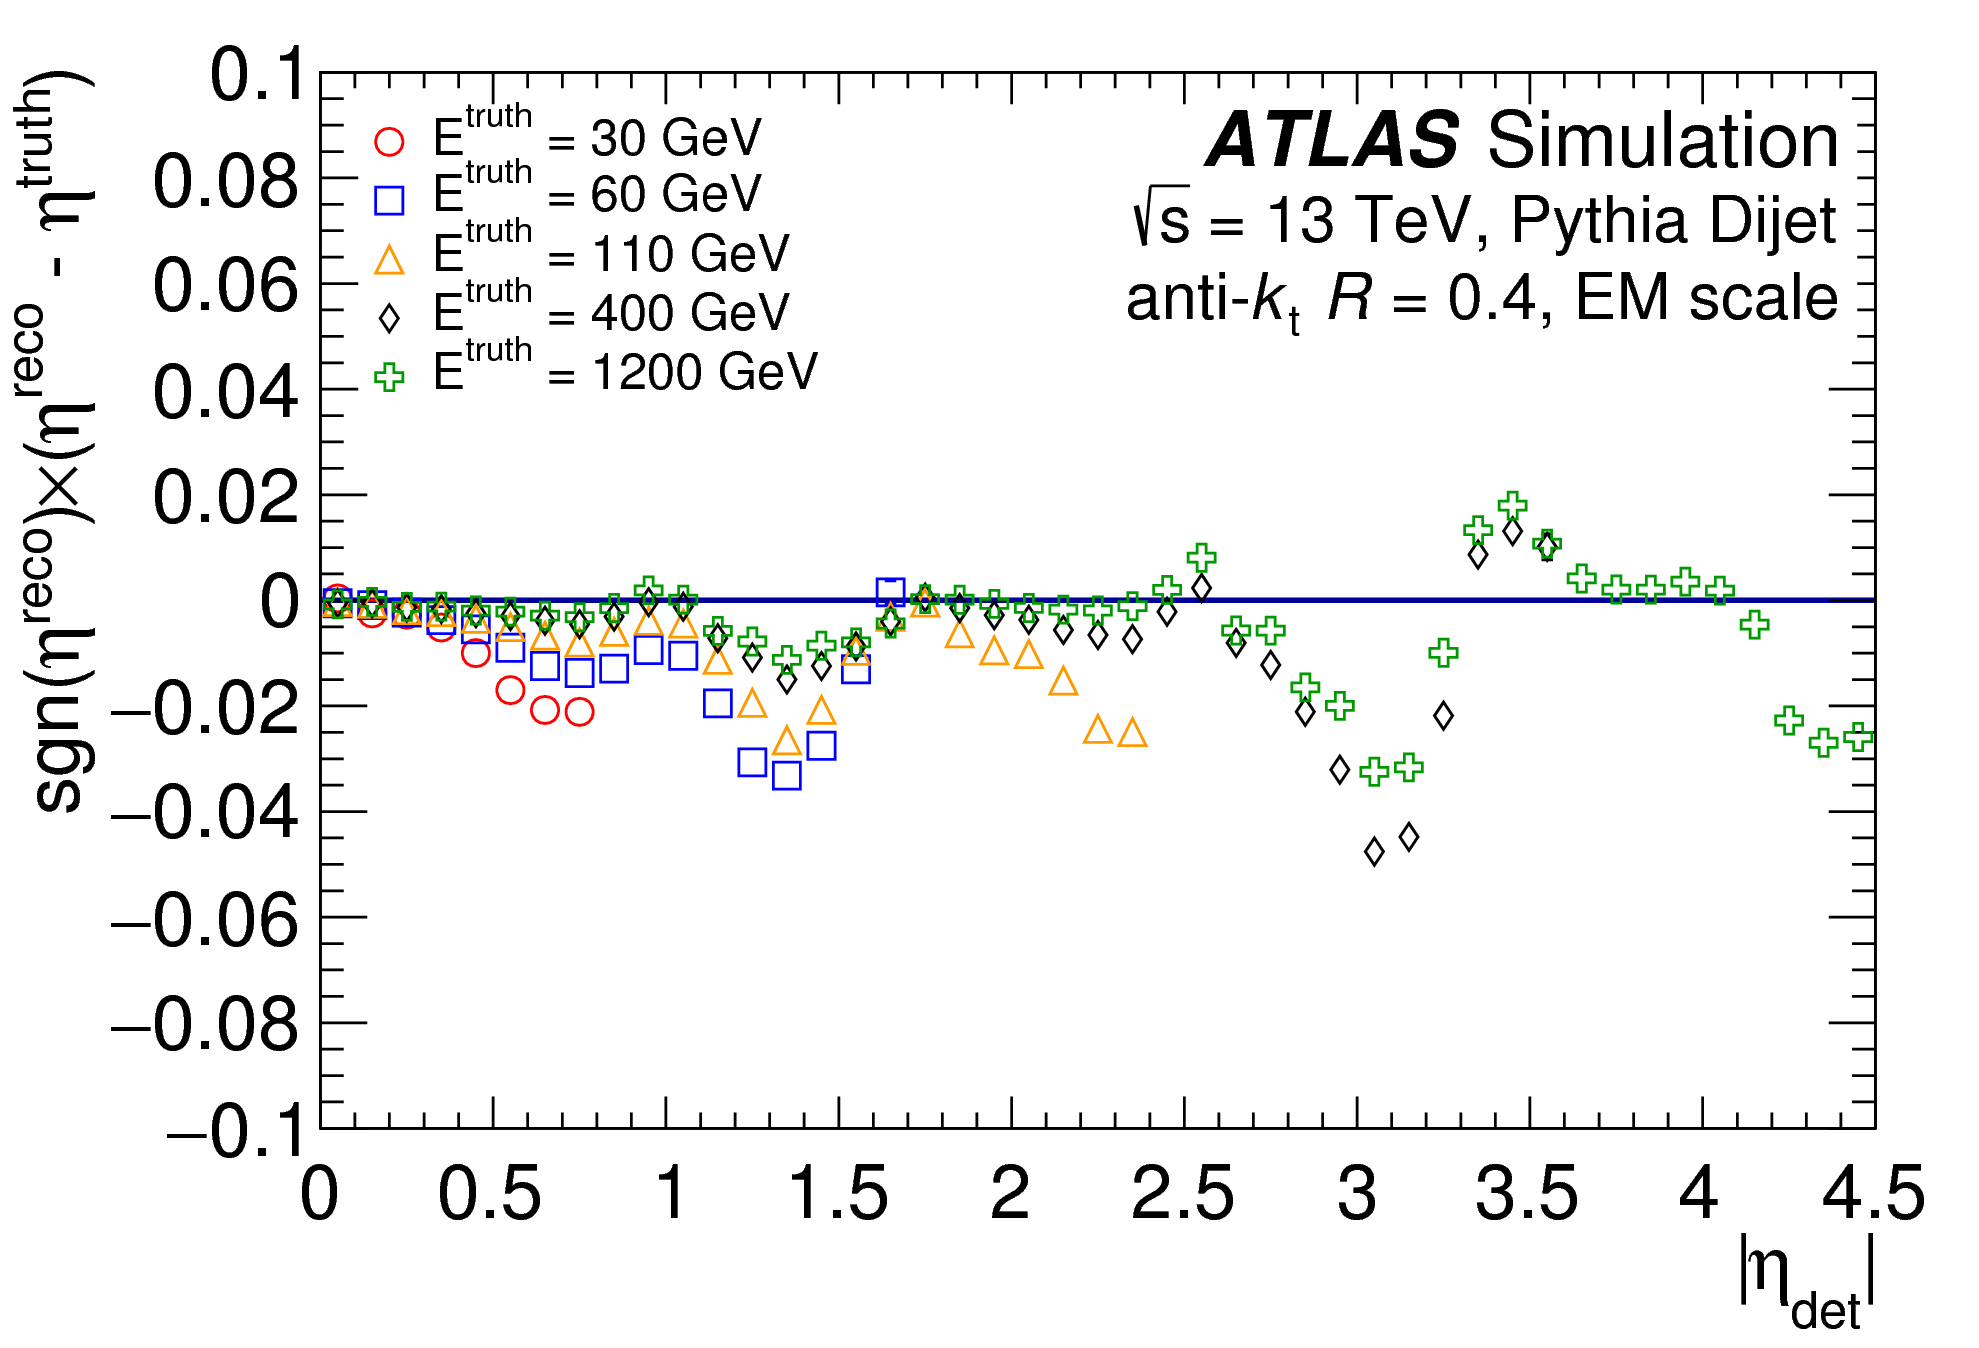
\includegraphics[width=0.48\textwidth]{figures/chapter3/jets/abs_jes_eta}
        \caption{
            \textbf{\textit{Left}}: Average energy response as a function of jet detector $\eta$, $\eta_{\text{det}}$.
            The colors correspond to different energy regimes for the particle-level jet to which the EM-scale
            reconstructed jet is matched. The inverse of the response is the final correction and can be seen to be
            largest for lower-\pT~jets.
            \textbf{\textit{Right}}: Difference in $\eta$ for the EM-scale reconstructed jet and the particle-level jet to which
            it is matched. The bias is clearly seen, with values typically negative, and it being largest
            for $\lvert \eta_{\text{det}} \rvert \sim 1.4$ $(\sim 3.1)$, corresponding to the barrel-endcap (endcap-forward)
            transition regions.
        }
        \label{fig:abs_jes_response}
    \end{center}
\end{figure}
\FloatBarrier

\subsubsection{Global Sequential Calibration}
\label{sec:jet_gsc}

The so-called Global Sequential Calibration (GSC) is a catch-all correction to account for remaining dependencies
of the EM+JES-scale jets on the jet shower shapes as well as fluctuations in the jet flavor composition and inter-jet energy distribution.
This correction improves the handling of fluctuations in the composition of the particles that initiate the jet; for example, correcting for the differences expected between quark- and gluon-initiated jets.
The former (quark-initiated) jets are typically more collimated with fewer, but higher-\pT, hadronic constituents.
The latter (gluon-initiated) jets typically contain many more, softer-\pT, particles and have wider transverse profiles
(and therefore do not traverse as far into the calorimeter).
The GSC has five stages, each following a numerical inversion of a corresponding jet response as in the case(s)
described in Section~\ref{sec:jet_eta_corr}, but are based on observables sensitive to the jet shower profile and growth
within the calorimeter as well as on the number and type of tracks associated with the reconstructed jet.
The use of tracking information from muons in this correction additionally helps with correcting the energy response of jets that
are not fully contained in the calorimeter but leak into the MS, so-called \textit{punch-through jets}.
Figure~\ref{fig:jet_punch_through} illustrates the concept of jet punch-through.

\begin{figure}[!htb]
    \begin{center}
        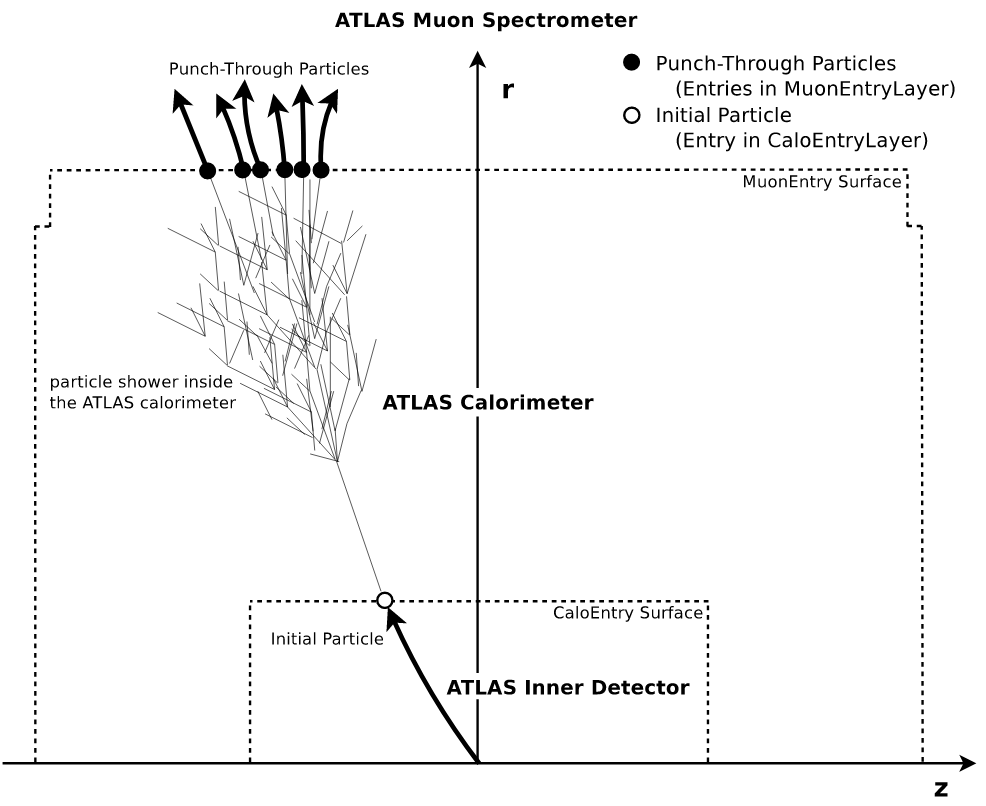
\includegraphics[width=0.6\textwidth]{figures/chapter3/jets/jet_punch_through}
        \caption{
            Illustration of jet punch-through.
            High momentum particles produced in the shower of an energetic jet within
            the hadronic calorimeter escape into the muon spectrometer, leaving detectable
            signatures in the muon chambers.
            It can be seen that energy and/or momentum may be left unaccounted for in the final event reconstruction or be assigned to separate muon objects as opposed to the
            initiating jet from which the punch-through particles arise.
            Such effects disrupt the proper
            assignment of energy-momentum to the jet and can spoil the overall momentum balance in the event.
        }
        \label{fig:jet_punch_through}
    \end{center}
\end{figure}

\subsubsection{In-situ Corrections}
\label{sec:jet_in_situ}

The last stage of the jet calibration accounts for remaining differences in the EM+JES jet response between data and simulation
and is primarily derived using events from data, as opposed to MC simulation.\footnote{In this case, the term `in-situ' means
that the corresponding corrections are derived using data, as opposed to using events from Monte-Carlo simulation.}
There are two classes of correction, the first being the so-called $\eta$-intercalibration step which corrects the
average response of forward jets ($0.8 < \lvert \eta \rvert < 4.5$) to that of well-measured central jets using dijet events
in which the two jets (the one in the forward region and the other in the central region) are back-to-back in $\phi$.
The second class of corrections is based on the method of balancing an EM+JES scale jet against a well-measured reference object.
The balance methods use only central jets ($\lvert \eta \rvert < 0.8$) and the choice of the reference object
provides the \pT~scale to which the response correction applies.
Balance methods using well-measured photons and $Z$ boson decays to leptons ($Z \rightarrow ee$ and $Z\rightarrow \mu \mu$)
as the reference objects are used to derive the response corrections for jets with \pT~up to 950\,\GeV.
Response corrections for jets covering \pT~ranges up to $2\,\TeV$ are derived using a multijet balance method
in which a high-\pT~central jet is balanced against a reference system of lower-\pT~jets.
The final response correction as a function of jet \pT~derived using these in-situ methods is shown in Figure~\ref{fig:jet_corr_insitu}.

\begin{figure}[!htb]
    \begin{center}
        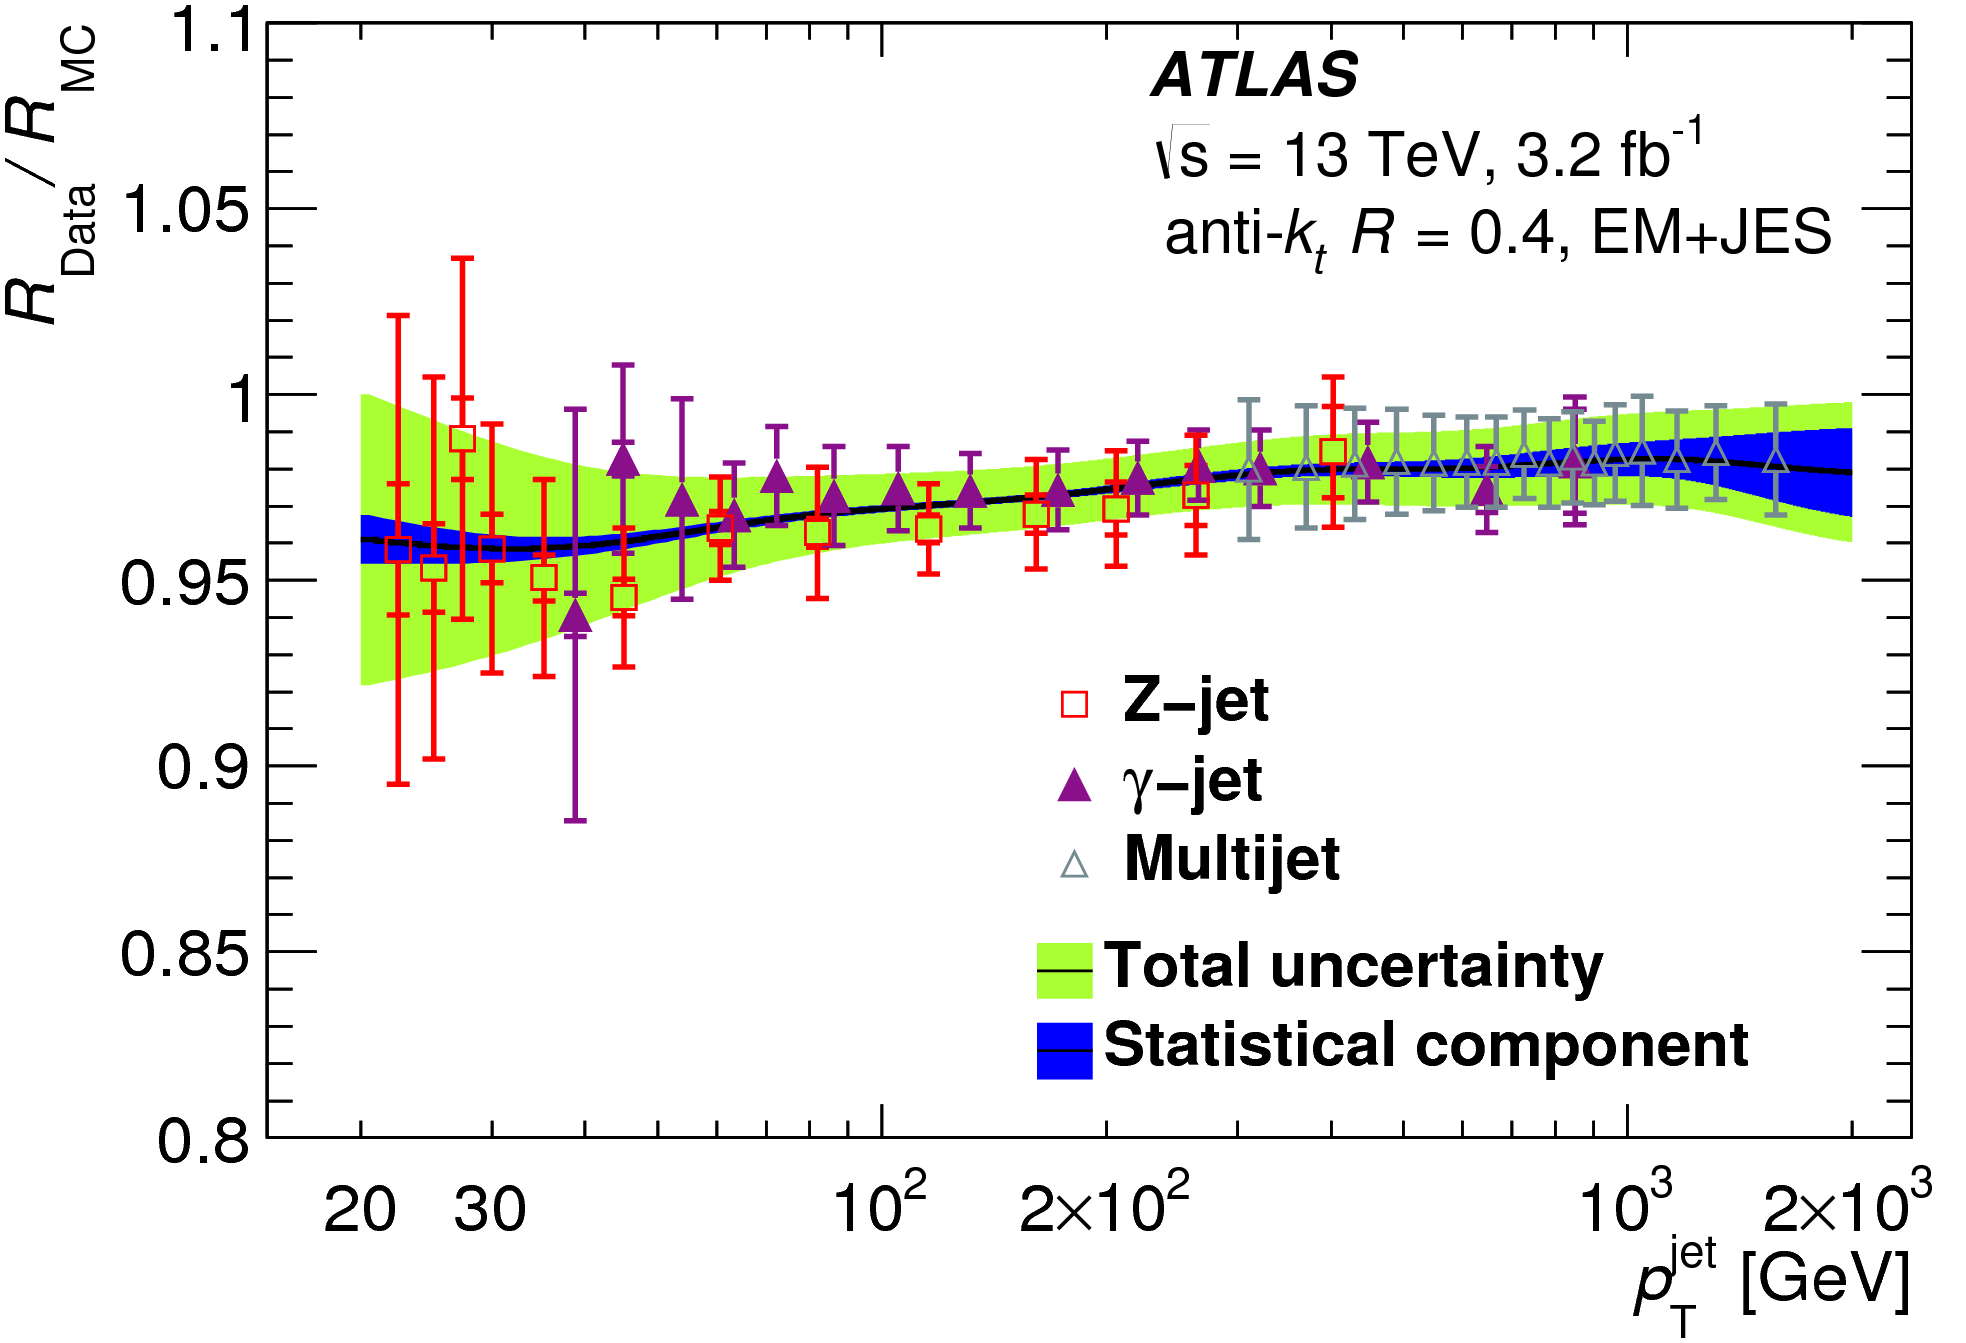
\includegraphics[width=0.7\textwidth]{figures/chapter3/jets/jet_corr_insitu}
        \caption{
            Ratio of the EM+JES jet response in data to that in MC simulation as a function of jet \pT.
            The different markers indicate the measurement contributions from the different
            reference-object used to derive the in-situ response corrections.
            The final response correction is given by the black line.
            The total uncertainty on the response is given by the green band and the blue band
            indicates only the statistical component of the uncertainty.
            Figure from Ref.~\cite{Aaboud:2017jcu}.
        }
        \label{fig:jet_corr_insitu}
    \end{center}
\end{figure}
\FloatBarrier
